\documentclass[12pt,a4paper]{article}
\usepackage[latin1]{inputenc}
\usepackage[english]{babel}
\usepackage{amsmath}
\usepackage{amsfonts}
\usepackage{amssymb}
\usepackage{graphicx}
\author{Pieterjan Bartels}
\title{Production and Development report}
\date{}
\begin{document}
\maketitle

This report will explain how the author came to his final submitted sequence of the two bouncing balls. It will describe the important concepts concisely, by going over all elements of the brief.\\

\section{Initial Idea}
Since the student is a basketball player and the project involves two bouncing balls, the student chose to make the sequence basketball themed. A lot of examples exist of basketball themed photographs, all having the basketball as most important element and the main lighting of the basketball arena turned off. The only light in the photograph is sunlight coming from a window or an open door. Examples can be seen in images \ref{img_ball},\ref{img_arena} and \ref{img_carter}. Sometimes some volumetric lighting can be seen in the pictures, due to dust particles floating around in the basketball arena.\\

Common in a lot of these representations is the dark area in the picture, contrasting with the front, lighted part. This is something that is used in movies, e.g. Legends of the guardian and is based on principles as Chiaroscuro, as very well explained and applied in [2], see image \ref{img_chiaro}. It's also used in horror movies, as the dark area represents a mystery: the viewer does not know what is in there, for example as in image \ref{img_conjuring}. The chosen object, the Darth Vader Lego figurine, was deemed to fit well with this look. The darkness and the shadows could work nicely with the somewhat creepy and evil connotations of Darth Vader.\\

The student chose to base his sequence on the aforementioned elements. The student made some sketches of what this could look like. In order to fit the Darth Vader figurine with the basketball size-wise, the student chose to oversize the figurine, as a visual hyperbole compared to the balls. That way the basketball or other ball could bounce off it in some way. The production was then aimed at achieving this look. Some different set-ups were tested out, e.g image \ref{img_sketch}, and in the end a full shot of the figurine was chosen, image \ref{img_earlyLight}. The different steps in this process are described in the next sections.\\

\section{Bouncing Balls}

The student chose two specific balls early on: an inflatable beachball and a basketball, both of which he had an example. Being a basketball player, he chose to bring some of his own experiences to life by animating a basketball falling on a wooden floor, as can be found on a typical basketball court. Rather than studying the behaviour of the chosen balls on online reference videos, the student made reference videos of both balls himself, on the right type of floor, see image \ref{img_reference}. These reference videos and the interaction with the real-life balls guided the student to make the on-screen behaviour of the balls realistic. One particular effect included in the videos was the change of direction due to the ball having a backspin. A ball with backspin changes direction on the first bounce, and loses his backspin in the process. \\

In order to analyze the principles of bouncing ball animation further, and learn the Maya interface at the same time, the student first made a short sequence based on a tutorial, resulting in quite cartoony ball, jumping up. This helped in understanding the basic principles of a ball falling due to gravity (constant acceleration leads to parabolic movement) and squash and stretch. After that, the movement of the actual balls was modeled in Maya, including backspin.\\

\section{Modeling the object.}
The object chosen by the student was a lego figurine of Darth Vader, seen in image \ref{img_vader}. The first step in the modeling was doing several exercises with maya, since the student was not familiar with the software.\\

Obviously, it was important to analyze the form of the figurine. For this, the student relied on observing the model, but also on looking up lego parts on the website lego.wikia.com [1]. This website includes part-numbers, which were used to find orthographic pictures of the figurine. Lego's own digital designer software came in handy for finding such pictures.

\section{Texturing and Materials}
For the materials of the objects in the sequence, the students chose to stay as close to the real world as possible, as was necessary for the wanted look. The student observed the existing materials, in order to match them to shader models available in Maya. The lego figurine was given a Blinn shading model, as it is plastic and shows specular highlights. The same goes for the beachball and the floor of the basketball court. The basketball and Vader's cape are non-specular.\\

The texture for the basketball court is based on BU's basketball court, the beach-ball texture was based on the actual beach-ball used while testing and the texture for Darth Vader's console is obviously based on the actual lego figurine. All three of these were self-made. The only texture that was not made by the student himself is the one for the basketball.\\

\section{Lighting \& rendering}
In order to achieve the dark and light contrast with light coming from a window, a directional key-light was used to mimic sunlight, combined with a polygonal object to make a window. An area light to get soft shadows, and an extra light to get the contours of the object a bit clearer complemented this. \\

In his initial plan, the student had planned to render the lights with a god ray (volumetric) effect, as seen in image \ref{img_carter}. However, the renderers in Maya unfortunately didn't have the tools to render this fast enough to allow several draft versions, although such algorithms do exist [5]. This volumetric effect was deemed unnecessary after testing the scene without it.

\section{Images}
In this section, some of the reference images and sketches are grouped together.

\begin{figure}
\center
\begin{minipage}{\textwidth}

\includegraphics[scale=0.3 ]{images/basketball_1.jpg} 
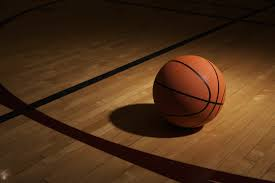
\includegraphics[scale=0.45 ]{images/basketball_2.jpg} 

\includegraphics[scale=0.3 ]{images/basketball_3.jpg} 
\end{minipage}
\caption{Typical basketball representations.}
\label{img_ball}
\end{figure}

\begin{figure}
\center
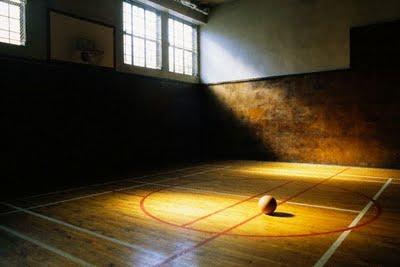
\includegraphics[scale=0.5]{images/court.png} 
\caption{Darkened court.}
\label{img_arena}
\end{figure}

\begin{figure}
\center
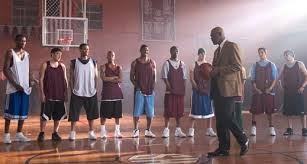
\includegraphics[scale=1]{images/carter.jpeg} 
\caption{Basketball court and lighting example for a basketball court. Notice the reflection in the court. Still from [3].}
\label{img_carter}
\end{figure}

\begin{figure}
\center
\begin{minipage}{\textwidth}
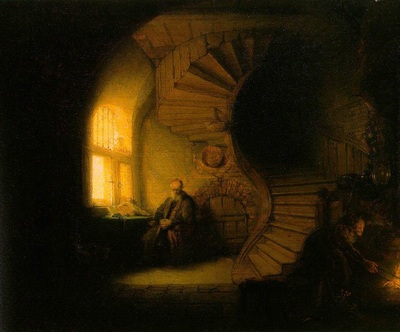
\includegraphics[scale=2 ]{images/chiaro_1.jpg} 
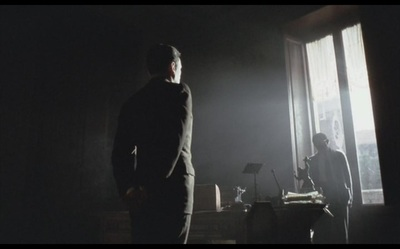
\includegraphics[scale=0.4 ]{images/chiaro_2.jpg} 
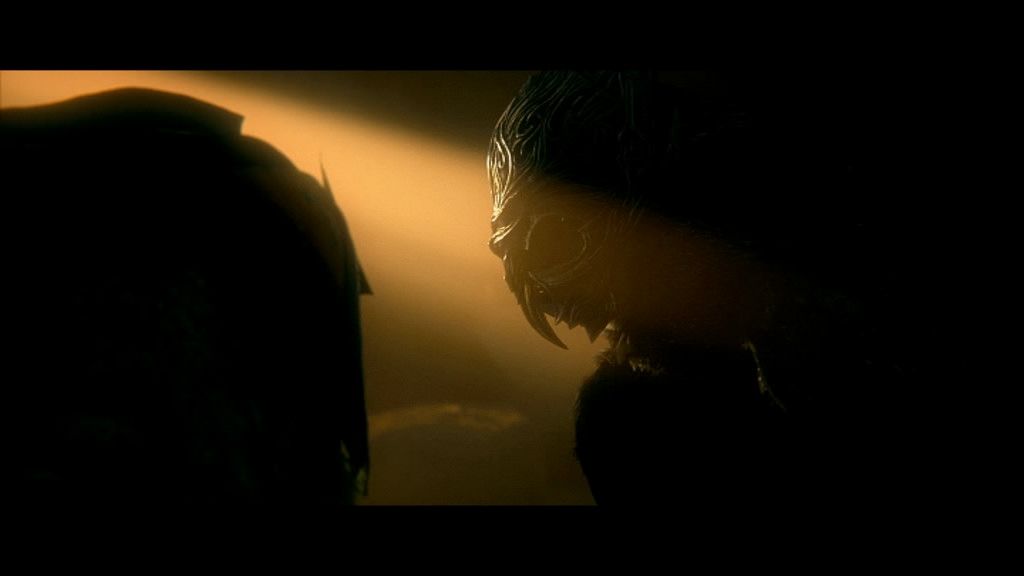
\includegraphics[scale=0.1 ]{images/chiaro_3.jpg} 
\end{minipage}
\caption{Dark and Light contrast (chiaroscuro) examples. The first image is an example from Rembrandt, the second one is from the movie 'Il Conformista', the third from 'Legend of the Guardians'. Images from [2].}
\label{img_chiaro}
\end{figure}

\begin{figure}
\center
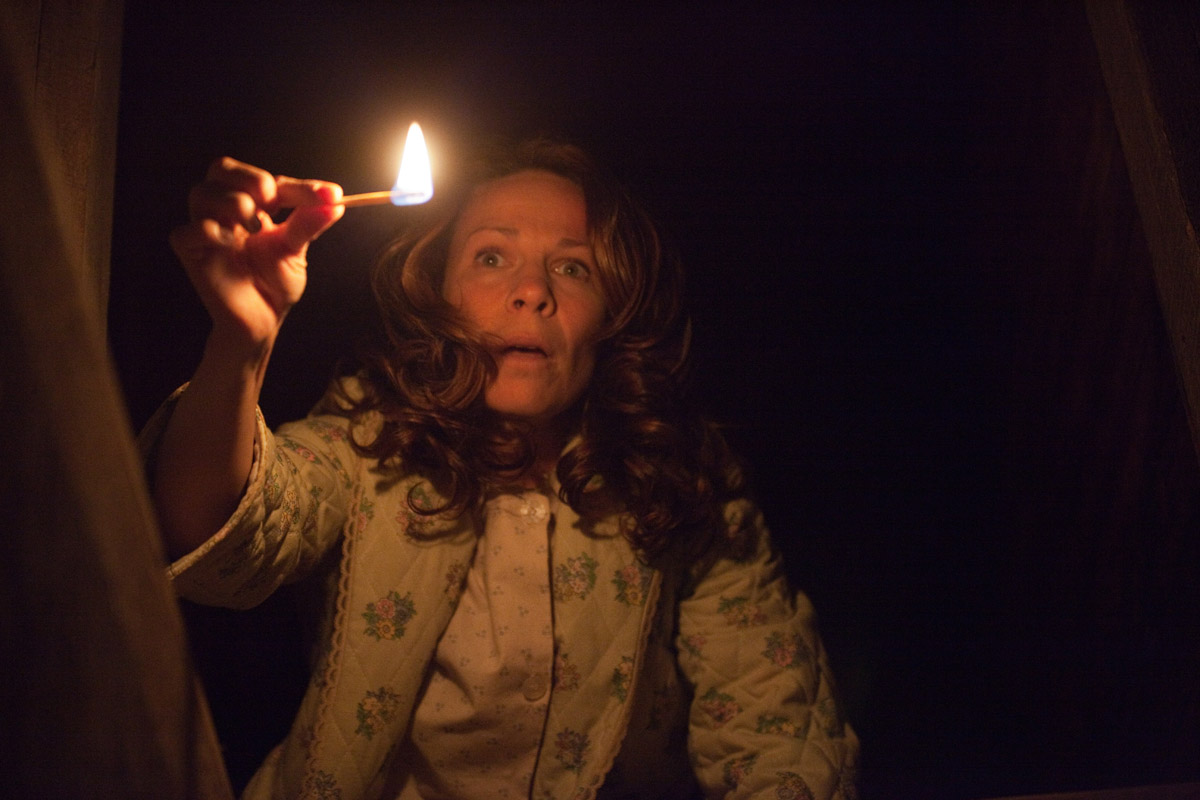
\includegraphics[scale=1]{images/conjuring.jpg} 
\caption{Dark and Light contrast in horror movie The conjuring [4].}
\label{img_conjuring}
\end{figure}

\begin{figure}
\center
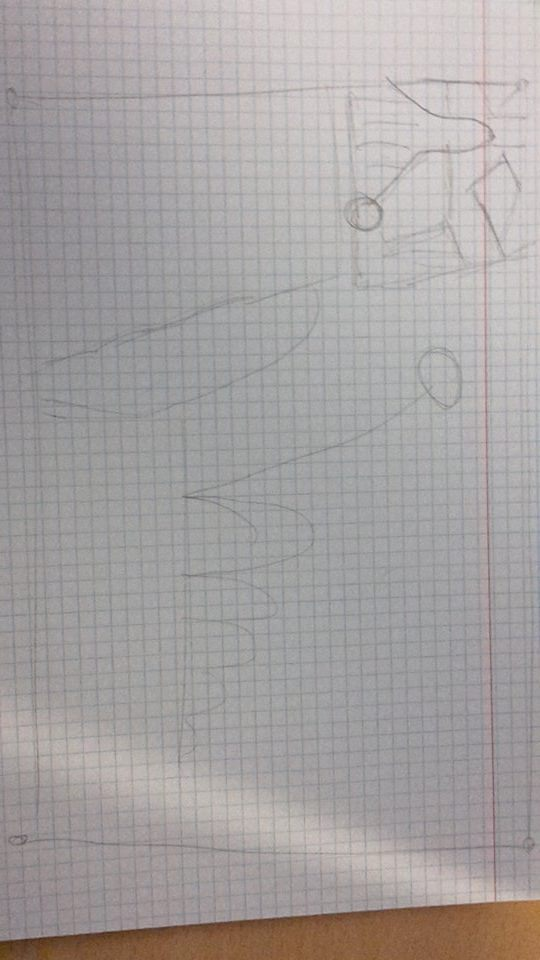
\includegraphics[ scale=0.25, angle=90 ]{images/old_sketch.jpg} 
\caption{Early stages showing the idea of a close-up of the figurine. Student felt that a full shot of the figurine worked better.}
\label{img_sketch}
\end{figure}

\begin{figure}
\center
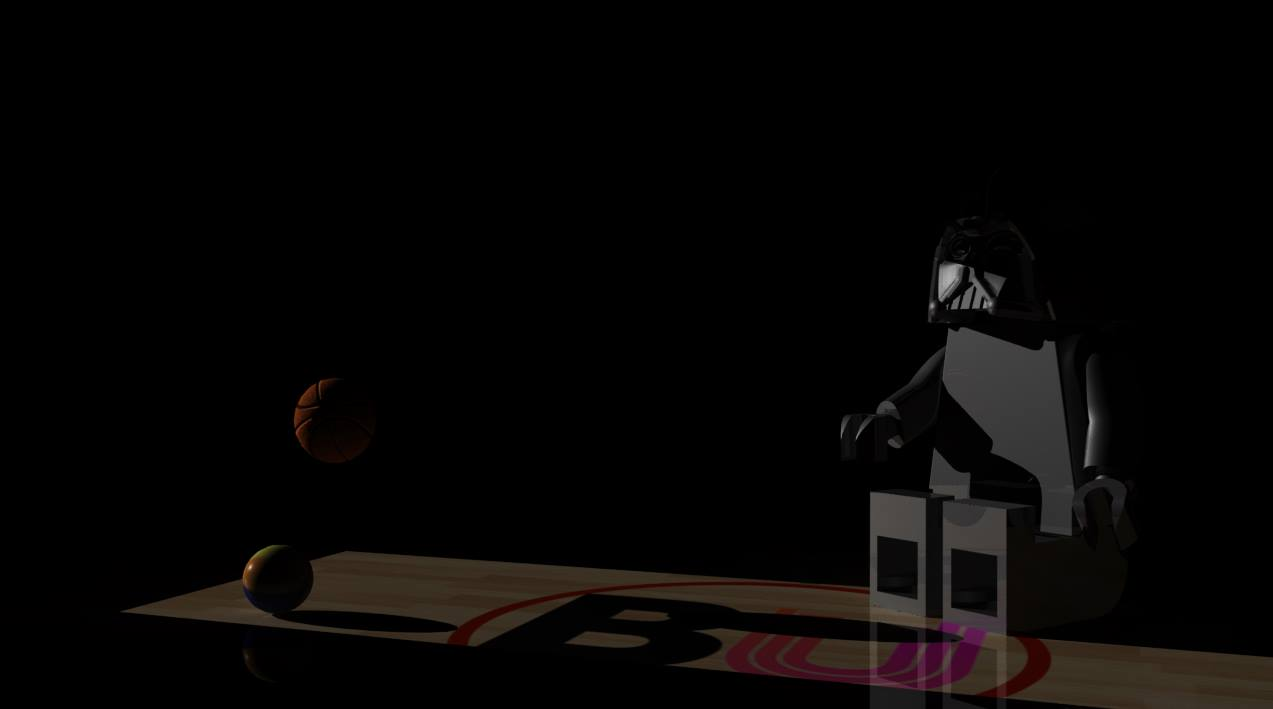
\includegraphics[scale=0.25 ]{images/earlyLighting.jpg} 
\caption{Final set-up with full shot and early lighting. While the lighting gives Darth Vader a more menacing look, there was not enough light on the balls, which were still the most important aspect of the assignment.}
\label{img_earlyLight}
\end{figure}

\begin{figure}
\center
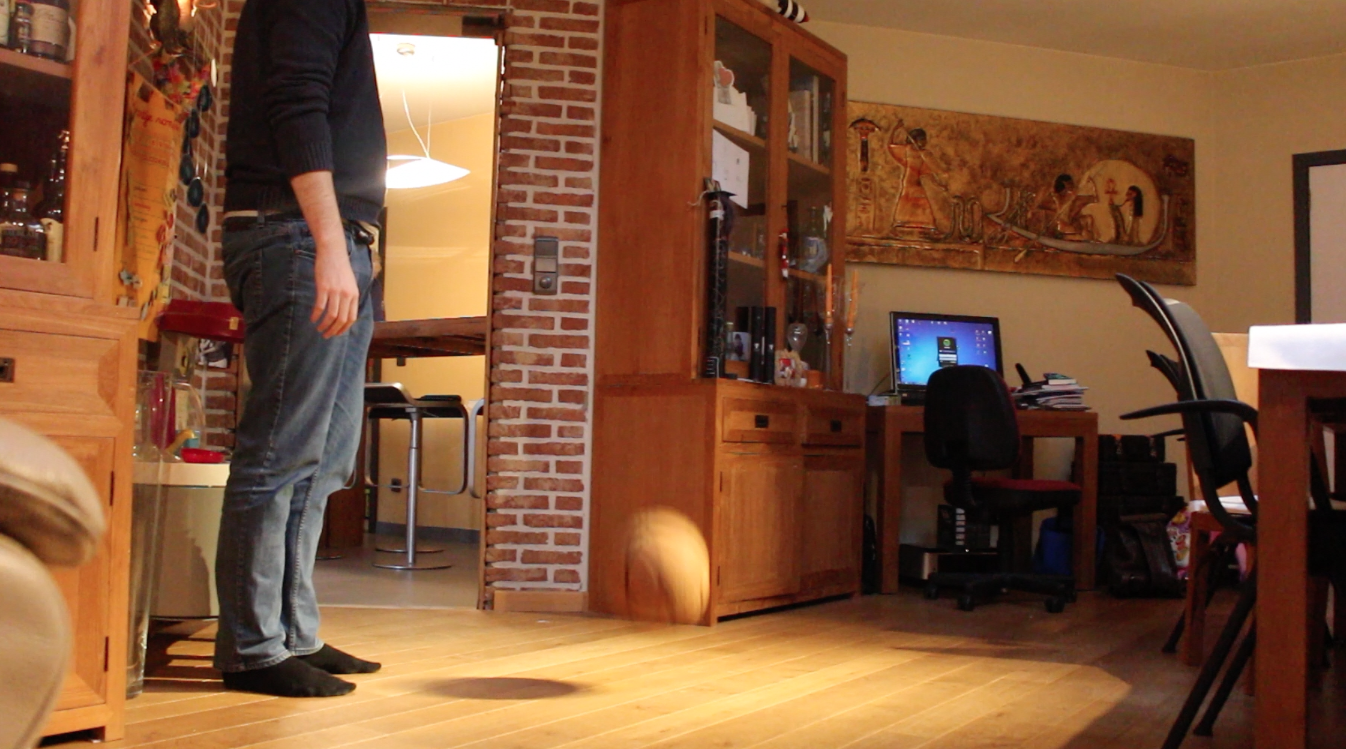
\includegraphics[scale=0.25 ]{images/reference.png} 
\caption{Screenshot of the self-made reference material.}
\label{img_reference}
\end{figure}

\begin{figure}
\center
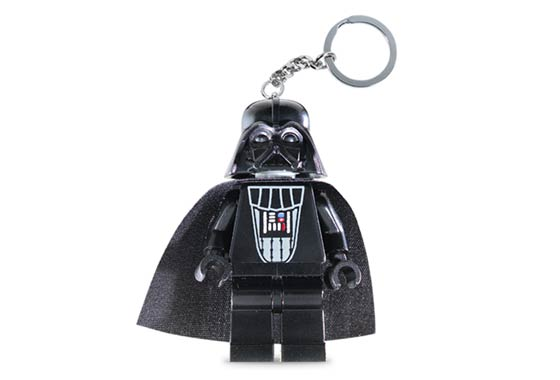
\includegraphics[scale=0.5]{images/vader.jpg} 
\caption{The modelled Lego figurine of Darth Vader.}
\label{img_vader}
\end{figure}

\begin{figure}
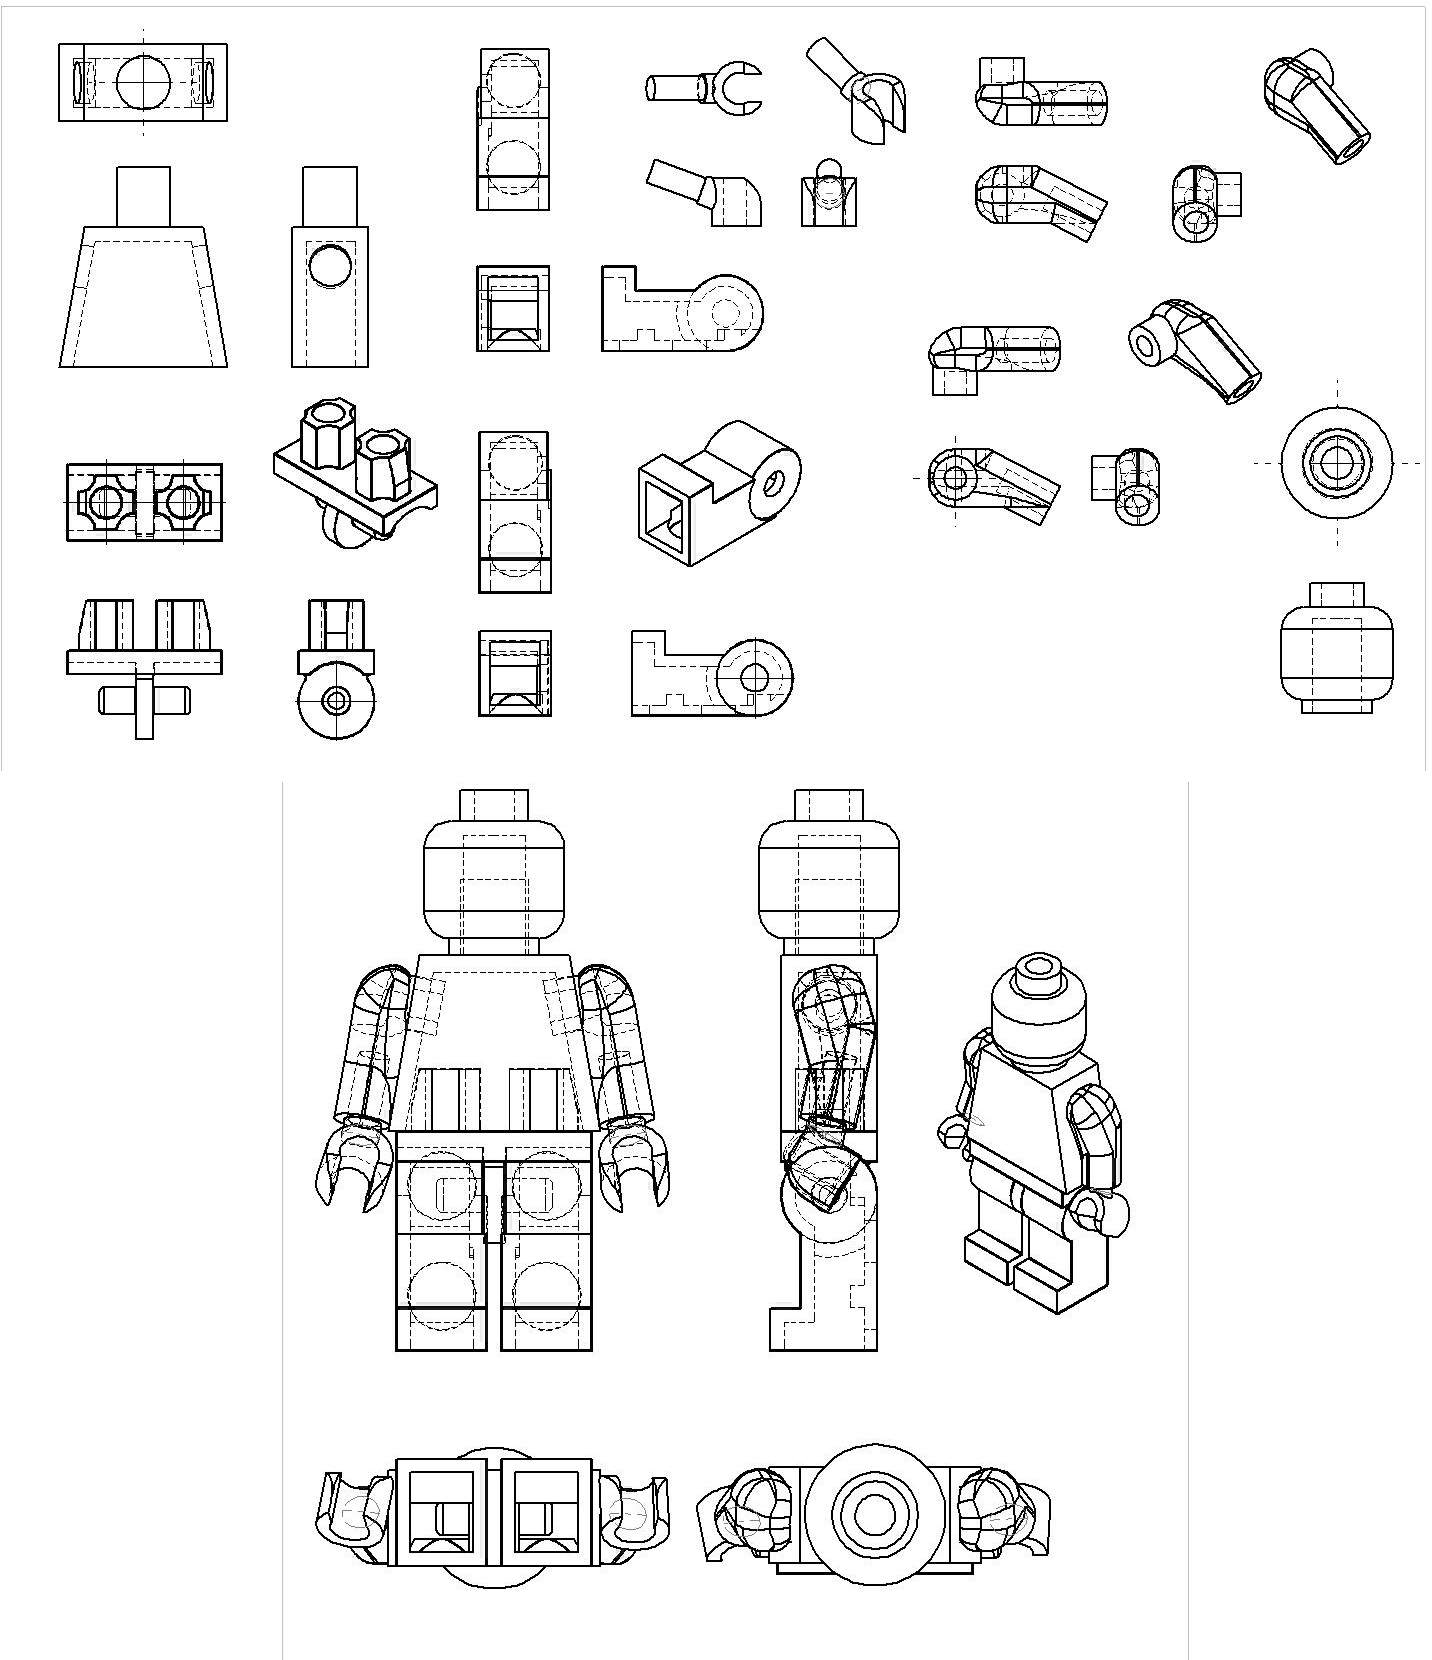
\includegraphics[scale=0.25]{images/BESTPICTURE.jpg} 
\caption{Reference material for the Lego Figurine body. Image from [1]}
\end{figure}

\clearpage
\section*{References}
\begin{description}
\item[1] Craig Palmer. 2014. Lego Wikia. [ONLINE] Available at:\\ http://lego.wikia.com/wiki/LEGO\_Wiki. [Accessed 15 January 15].
\item[2] Craig Welsh. 2014. The Cinematography of "Legend of the Guardians". [ONLINE] Available at: \\ http://www.expandedcinematography.com/the-cinematography-of-legend-of-the-guardians.html. [Accessed 15 January 15].
\item[3] Coach Carter, 2005. [DVD] Thomas Carter, USA: Paramount Pictures.
\item[4] The Conjuring, 2013. [DVD] James Wan, USA: Warner Bros. Pictures.
\item[5] Jan Novak, Derek Nowrouzezahrai, Carsten Dachsbacher, Wojciech Jarosz. 2012, Virtual Ray Lights for Rendering Scenes with Participating Media. In: \textit{the 11th ACM SIGGRAPH/Eurographics Symposium on Computer Animation (SCA '12)}.
\end{description}

\end{document}